\section{Atomic Operations}

\subsection{Atomic Operations}
\begin{frame}
\frametitle{Atomic Operations}
	
\includegraphics[width=0.9\textwidth]{img/atom.jpg}
\end{frame}


\subsection{Atomic operations using with}
\begin{frame}[fragile]
\frametitle{Atomic operations using with}

\begin{lstlisting}[style=pythoncode]
# Fix population from absolute to relative
layer.startEditing()
for feat in layer.getFeatures():
	feat['population'] = feat['population'] / feat['area']
	layer.updateFeature(feat)
layer.commitChanges()
layer.stopEditing()
\end{lstlisting}
\pause
\begin{lstlisting}[style=pythonoutput]
ZeroDivisionError: division by zero
\end{lstlisting}

\end{frame}

\subsection{Atomic Operations}
\begin{frame}
\frametitle{Atomic Operations}
	
\includegraphics[width=0.9\textwidth]{img/atombombe.jpg}
\end{frame}

\subsection{Atomic operations using "with"}
\begin{frame}[fragile]
\frametitle{Atomic operations using "with"}
\begin{itemize}
	\item Only part of the features are modified
	\item The layer may or may not be in edit state any more
\end{itemize}
\end{frame}

\subsection{Atomic operations using "with"}
\begin{frame}[fragile]
\frametitle{Atomic operations using "with"}
Let's introduce "with"
\end{frame}

\subsection{Atomic operations using "with"}
\begin{frame}[fragile]
\frametitle{Atomic operations using "with"}

\begin{lstlisting}[style=pythoncode]
# Fix population from absolute to relative
with edit(layer):
	for feat in layer.getFeatures():
		feat['population'] = feat['population'] / feat['area']
		layer.updateFeature(feat)
# Changes are committed automatically if no error occurred
\end{lstlisting}
\pause
\begin{lstlisting}[style=pythonoutput]
# Or if an error occurs, no changes are applied at all
ZeroDivisionError: division by zero
\end{lstlisting}

\end{frame}

\subsection{Atomic Operations}
\begin{frame}
\frametitle{Atomic Operations}
	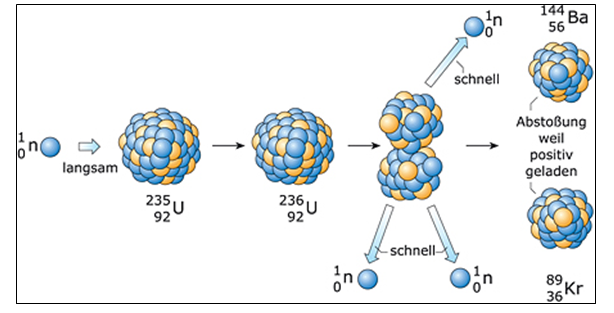
\includegraphics[width=0.9\textwidth]{img/controlled-chain-reaction.png}
\end{frame}
